\documentclass[12pt,a3paper]{article}
\usepackage[utf8]{inputenc}
\usepackage[spanish,es-sloppy]{babel}
\usepackage{amsmath}
\usepackage{amsfonts}
\usepackage{amssymb}
\usepackage{graphicx}
\usepackage{tcolorbox}
\usepackage{here}
\usepackage[left=1.8cm,right=1.8cm,top=1.5cm,bottom=1.5cm]{geometry}
\usepackage{verbments}
%\definecolor{fondo1}{rgb}{0.9764, 0.9764, 0.9762}
%\definecolor{fondo2}{rgb}{0.1647, 0.4980, 0.7}
\definecolor{fondo1}{rgb}{0.88, 0.88, 0.88}
\definecolor{fondo2}{rgb}{0.15, 0.15, 0.5}
\author{Josue Huaroto Villavicencio - 20174070I\\Sección: E}
\title{4$^{\circ}$ Práctica de Cálculo por Elementos Finitos - MC516}
\begin{document}
\fvset{frame=bottomline, framerule=0.02cm,numbers=left, numbersep=8pt}
\plset{language=python,texcl=true,listingnamefont=\sffamily\bfseries\color{white},captionbgcolor=fondo2, bgcolor=fondo1,listingname=\textbf{Código}, captionfont=\sffamily\color{white},fontsize=\large}
\tcbset{colframe=black!50!gray,colback=gray!20,colupper=black,fonttitle=\bfseries,nobeforeafter,center title}
\maketitle
%\tableofcontents
\section{Diagrama de flujo}
\begin{figure}[H]
    \centering
    \includegraphics[scale = 1.75]{Flow.pdf}
    \caption{Diagrama de flujo}
\end{figure}
\section{Ejecución del código}
Del solver principal, se modifica algunas funciones para implementar ahora los elementos de la armadura en 3D.
\begin{pyglist}[language=python,caption={Cálculo de la longitud y el ángulo entre nodos},style=pastie]
def AllAngle(f,s):
    L = DistanceNodes(f,s)
    C = []
    for i in range(3):
        C.append((s[i]-f[i])/L)
    C = np.arccos(np.array(C))
    return [C,L]

def DistanceNodes(f,s):
    return np.sqrt((s[0]-f[0])**2+(s[1]-f[1])**2+(s[2]-f[2])**2)

def SingleAngle(f,s):
    if(s[0] == f[0]):
        aux = np.pi/2
        if(s[1] < f[1]):
             aux *= -1
        return aux
    else:
        aux = np.arctan((s[1]-f[1])/(s[0]-f[0]))
        
    if(aux < 0 and s[1] > f[1]):
        aux += np.pi
        
    if(s[1] < f[1]):
        aux += np.pi
        if(s[0] > f[0]):
            aux += np.pi
    return aux
\end{pyglist}
Ahora, es necesario modificar la inserción de las matrices de rigidez de los elementos a la matriz de rigidez global.
\begin{pyglist}[language=python,caption={Ensamble de la matriz de rigidez},style=pastie]
def AssemblyStiffness(nStiffnessMatrix,k,i,j):
    for p in range(0,3):
        for m in range(0,3):
            nStiffnessMatrix[3*i+p][3*i+m] += k[p][m]
            nStiffnessMatrix[3*i+p][3*j+m] += k[p][3+m]
            nStiffnessMatrix[3*j+p][3*i+m] += k[p+3][m]
            nStiffnessMatrix[3*j+p][3*j+m] += k[p+3][3+m]
 
def Initialize(nStiffnessMatrix,nU,nF):
    for i in range(0,Nodes):
        nU[i][0] = 0
        nF[i][0] = 0
        
    for i in range(0,NumberOfElement):
        AssemblyStiffness(nStiffnessMatrix,K[i],int(Elements[i][0]),int(Elements[i][1]))
\end{pyglist}
Todos los demás elementos del código permanecen igual; ahora solo se necesita definir las condiciones del problema a resolver.
\begin{pyglist}[language=python,caption={Condiciones del problema},style=pastie]
NodesCondition = []
Nodes = 12
Nodes *= 3
NumberOfElement = 33

E = 2.1e5 #MPA
A = np.pi*25*25 #mm$^2$
K = []
L = []
P_A = 10000 #N
P_B = 8000 #N
l1 = 600 #mm
l2 = 500#mm
alpha = 30*np.pi/180
beta = 70*np.pi/180

PosNodes = np.array([(0,0,0),(l1,0,0),(2*l1,0,0),(3*l1,0,0),
                    (l1,-l1*np.tan(alpha),0),(2*l1,-l1*np.tan(alpha),0),
                    (0,0,-l2),(l1,0,-l2),(2*l1,0,-l2),(3*l1,0,-l2),
                    (l1,-l1*np.tan(alpha),-l2),(2*l1,-l1*np.tan(alpha),-l2)])

Elements = np.array([(0,1),(0,4),(0,6),(0,10),
                     (1,2),(1,4),(1,6),(1,7),(1,8),(1,10),
                     (2,3),(2,4),(2,5),(2,8),(2,10),(2,11),
                     (3,5),(3,8),(3,9),(3,11),
                     (4,5),(4,10),
                     (5,10),(5,11),
                     (6,7),(6,10),
                     (7,8),(7,10),
                     (8,9),(8,10),(8,11),
                     (9,11),
                     (10,11)])

for i in range(0,NumberOfElement):
    L.append(AllAngle(PosNodes[Elements[i][0]],PosNodes[Elements[i][1]]))

L = np.array(L)

for i in range(0,NumberOfElement):
    l = L[i][1]
    angles = np.cos(L[i][0])
    aux = np.zeros((6,6))
    w = np.zeros((3,3))
    
    for j in range(0,3):
        for k in range(0,3):
            w[j][k] = angles[j]*angles[k]
            
    for k in range(6):
        for j in range(6):
            s = 1
            
            if k >= 3:
                s *= -1
                
            if j >= 3:
                s *= -1
            aux[k][j] = w[k%3][j%3]*s
            
    aux = aux*E*A/l
    K.append(aux)


StiffnessMatrix = np.zeros((Nodes,Nodes))

U = np.zeros(Nodes).reshape(Nodes,1)
F = np.zeros(Nodes).reshape(Nodes,1)

Initialize(StiffnessMatrix,U,F)

#Node in UBoundary = Node*3+(x=0,y=1,z=2)
UBoundaryCondition(U,0,3*0+0) #Nodo 0 en X
UBoundaryCondition(U,0,3*0+1) #Nodo 0 en Y
UBoundaryCondition(U,0,3*0+2) #Nodo 0 en Z

UBoundaryCondition(U,0,3*6+0) #Nodo 6 en X
UBoundaryCondition(U,0,3*6+1) #Nodo 6 en Y
UBoundaryCondition(U,0,3*6+2) #Nodo 6 en Z

UBoundaryCondition(U,0,3*3+1) #Nodo 3 en Y
UBoundaryCondition(U,0,3*3+2) #Nodo 3 en Z

UBoundaryCondition(U,0,3*9+1) #Nodo 9 en Y
UBoundaryCondition(U,0,3*9+2) #Nodo 9 en Z

FBoundaryCondition(F,-P_A/2,3*4+1) #Nodo 4 en Y
FBoundaryCondition(F,-P_A/2,3*10+1) #Nodo 10 en Y

FBoundaryCondition(F,P_B*np.sin(beta)/2,3*5+0) #Nodo 5 en X
FBoundaryCondition(F,P_B*np.sin(beta)/2,3*11+0) #Nodo 11 en X

FBoundaryCondition(F,-P_B*np.cos(beta)/2,3*5+1) #Nodo 5 en Y
FBoundaryCondition(F,-P_B*np.cos(beta)/2,3*11+1) #Nodo 11 en Y


U,F=Solve(StiffnessMatrix,U,F)

nU = np.zeros((U.shape[0]//3,3))
nF = np.zeros((U.shape[0]//3,3))

for i in range(U.shape[0]//3):
    for j in range(3):
        nU[i][j] = U[3*i+j][0]
        nF[i][j] = F[3*i+j][0]

print("Stiffness Matrix:\n",StiffnessMatrix,'\n')
print("Displacements:\n",nU,'\n')
print("Forces:\n",nF)
\end{pyglist}
La notación para las condiciones del problema es muy similar a los problemas anteriores de barras, siendo la diferencia más notable que no hay una relación directa entre nodos y cantidad de elementos.\\
La representación de la armadura es:
\begin{figure}[H]
    \centering
    \includegraphics[scale=1.2]{truss2.pdf}
    \caption{Armadura 3D}
\end{figure}
\section{Resultados del problema}
Al finalizar la ejecución del solver, obtenemos la matriz de rigidez, las fuerzas y desplazamientos:
\begin{figure}[H]
    \centering
    %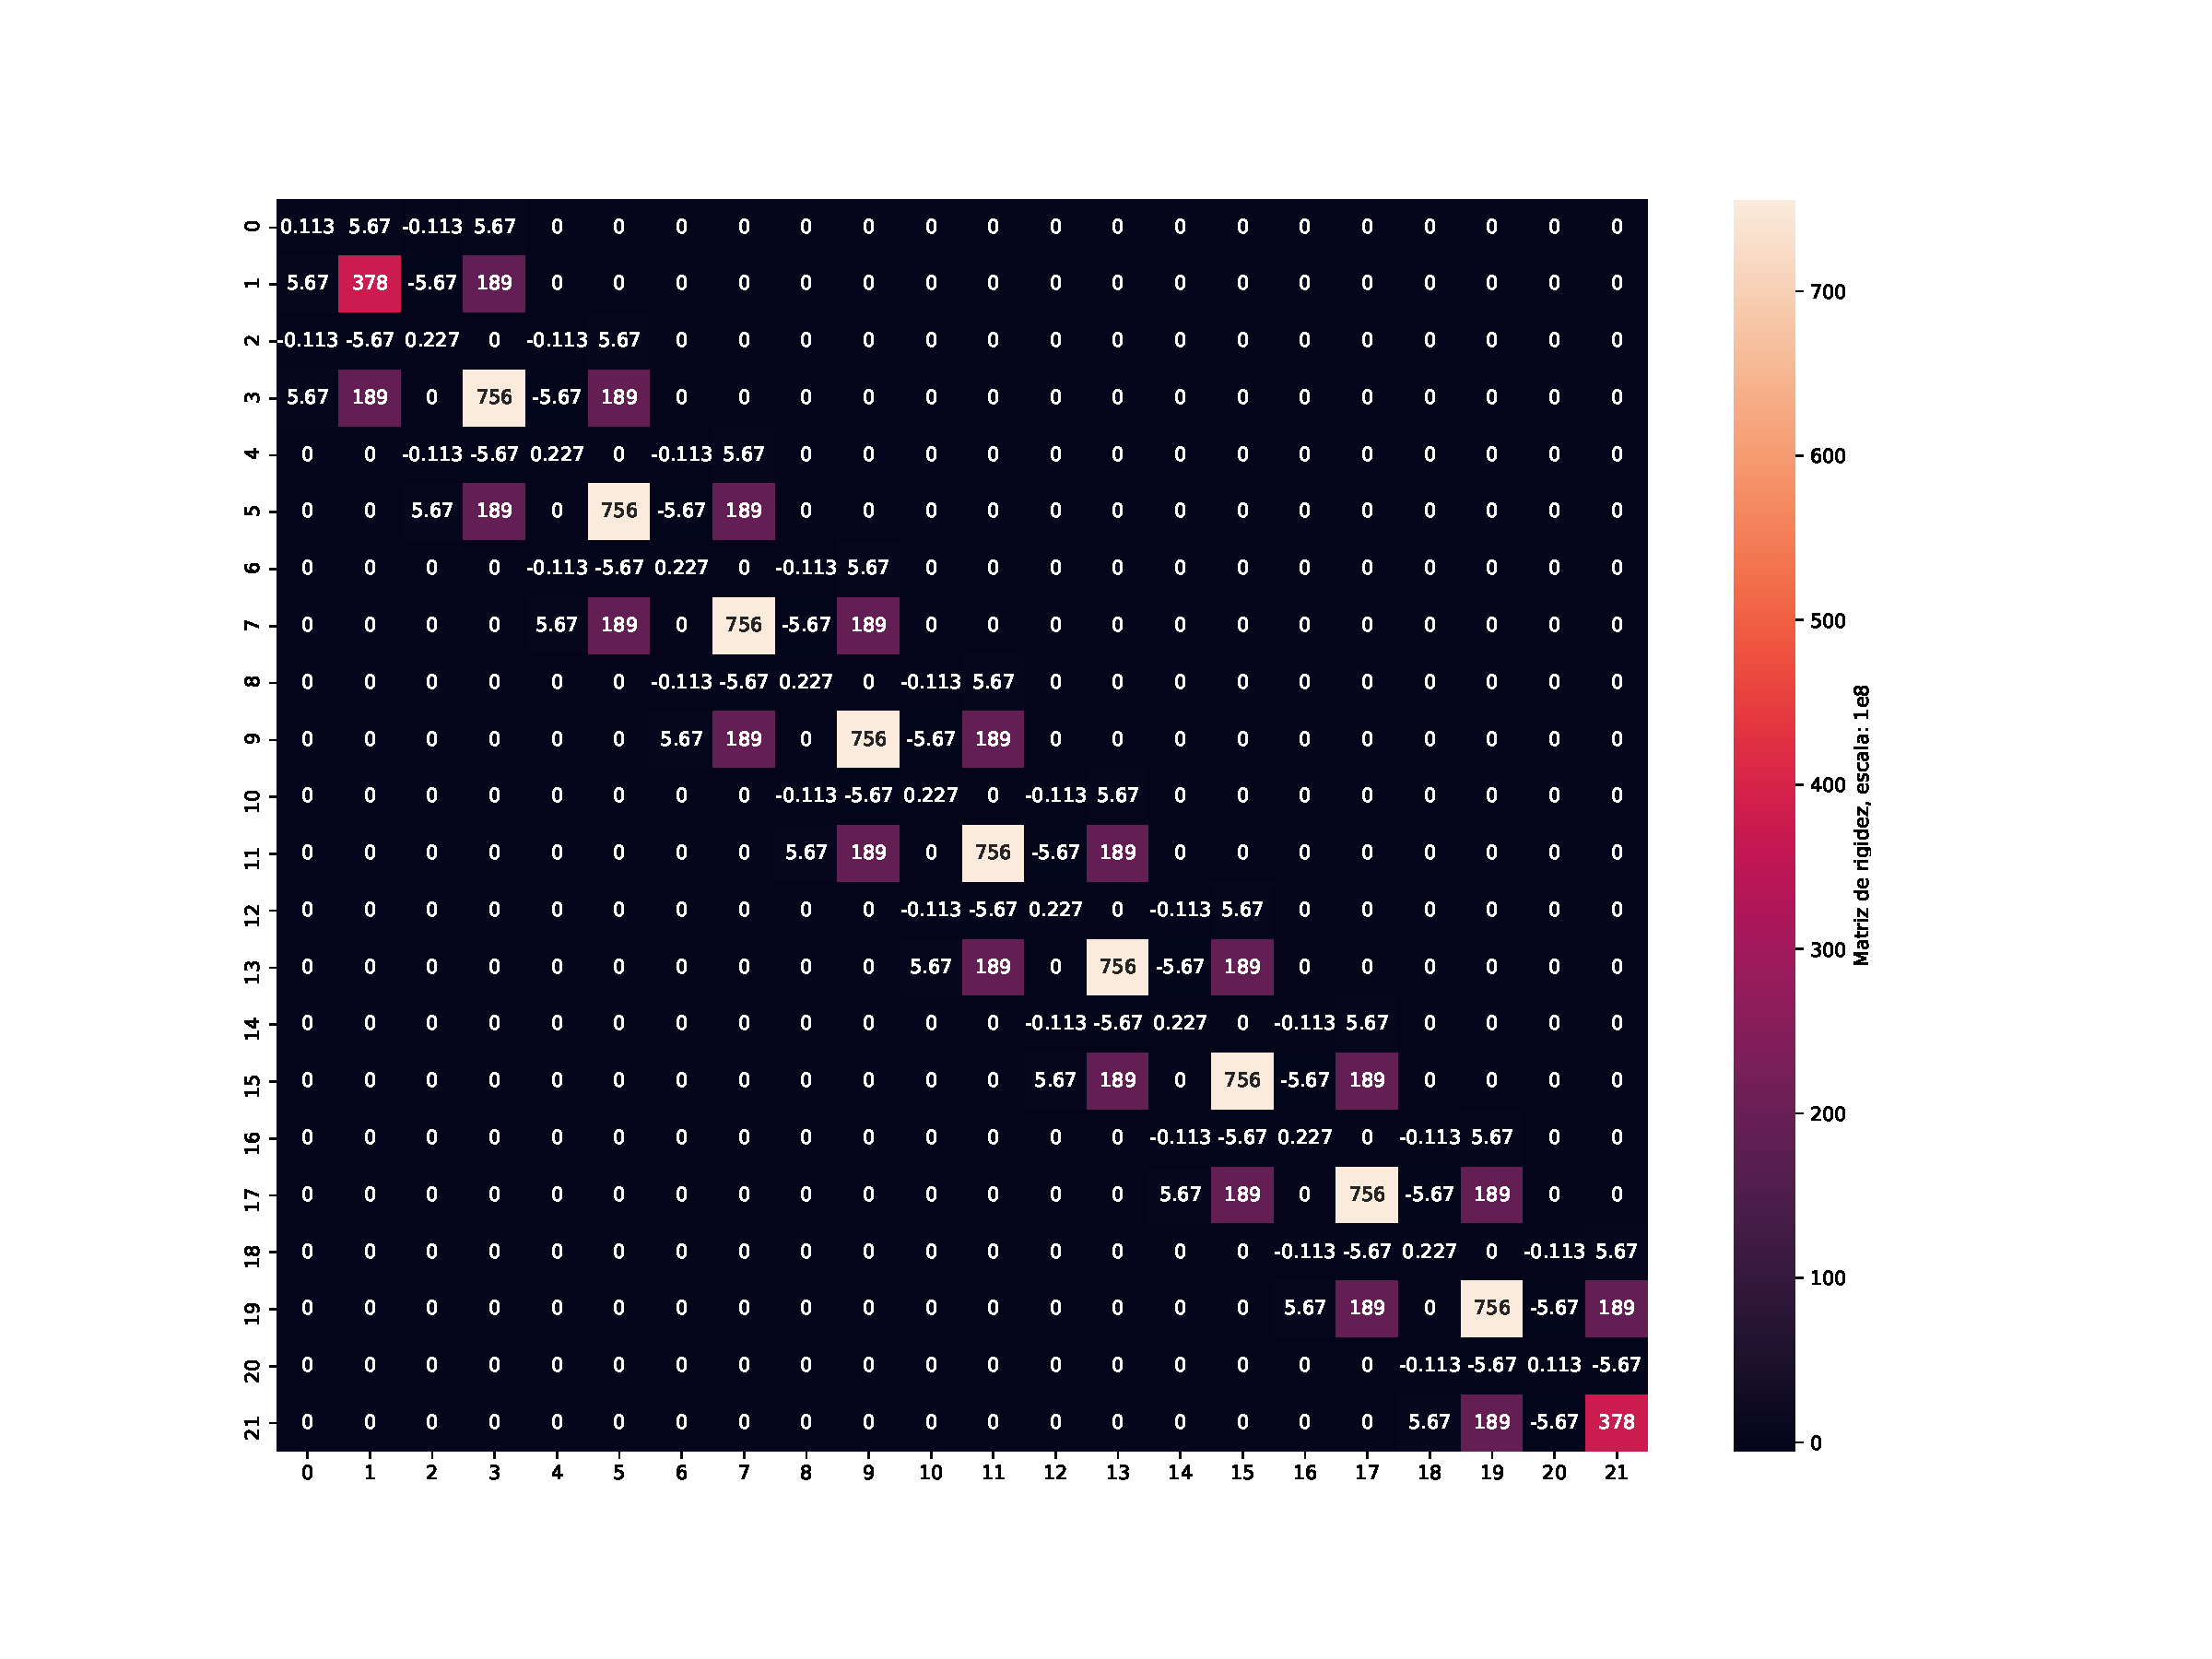
\includegraphics[height=11cm,width=17cm]{stiffness.pdf}
    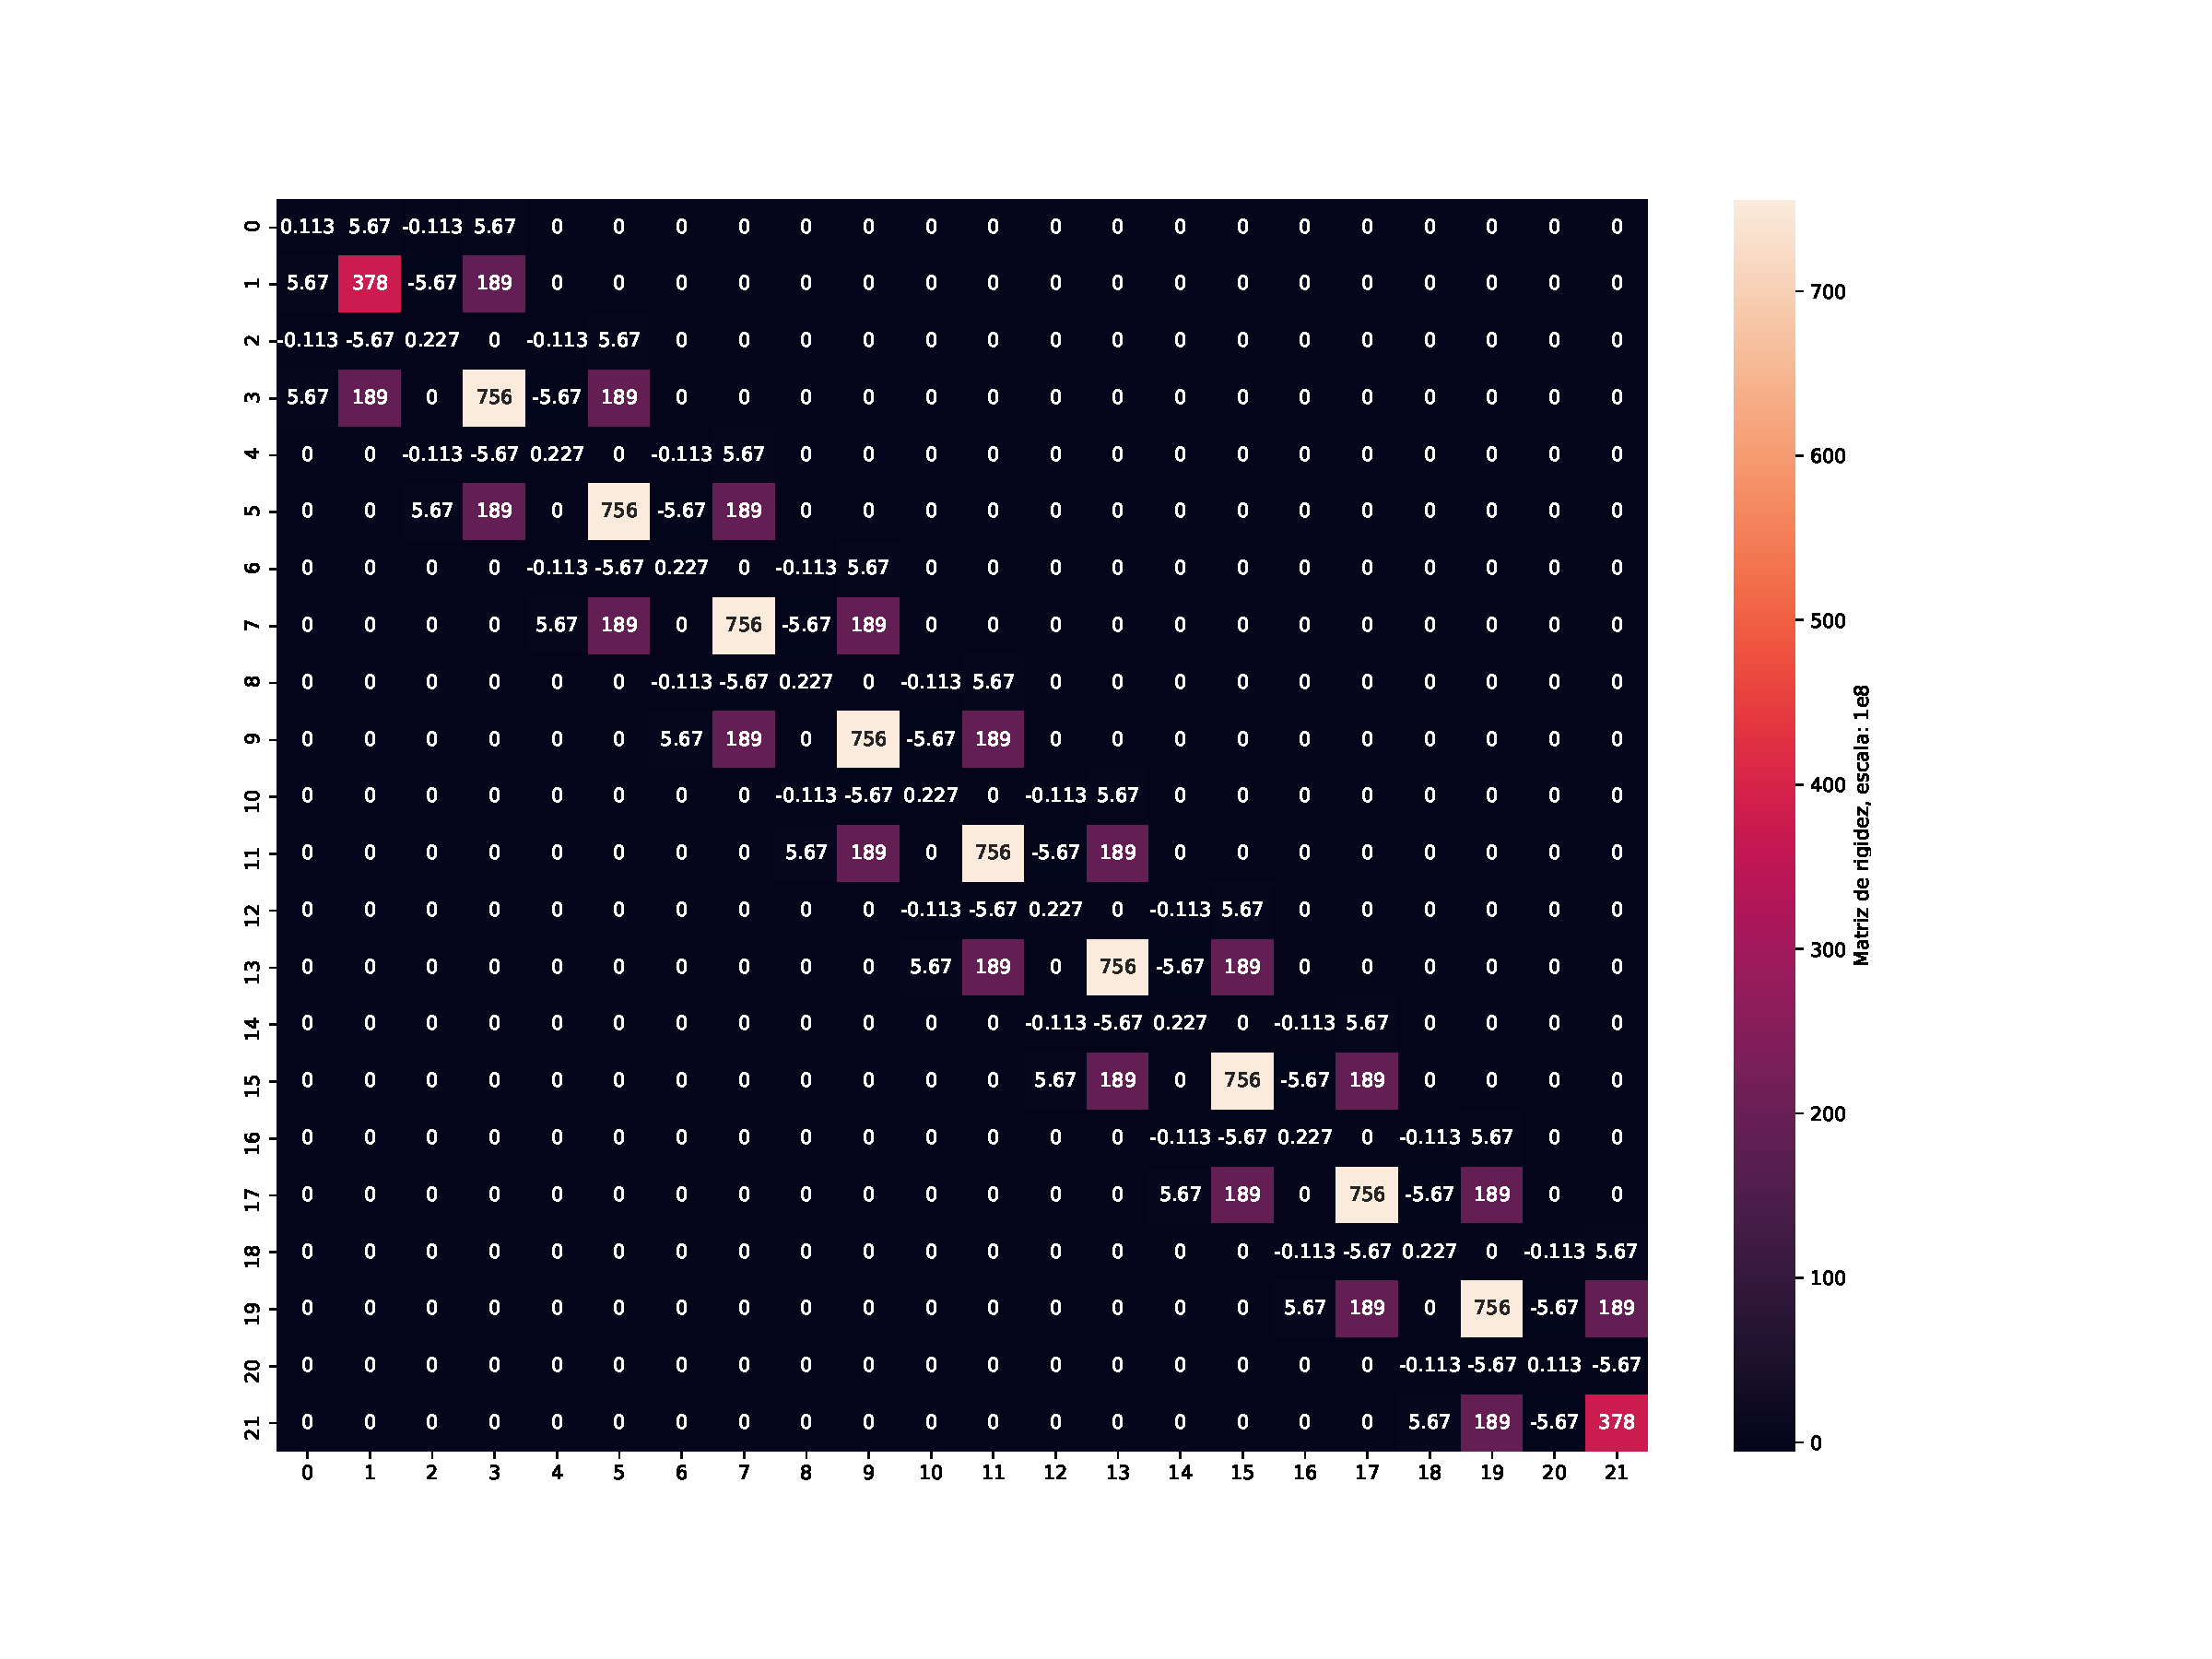
\includegraphics[scale=0.575]{stiffness.pdf}
    \caption{Matriz de rigidez}
\end{figure}
\begin{figure}[H]
    \centering
    \includegraphics[width=11cm,height=11.8cm]{displacements.pdf}
    \includegraphics[width=11cm,height=11.8cm]{forces.pdf}
    \includegraphics[width=9.5cm,height=9.8cm]{f_r.pdf}
    \caption{Desplazamientos y fuerzas}
\end{figure}
Cada desplazamiento y fuerza corresponde a un nodo en una dirección ($x$, $y$ o $z$); por lo que al nodo $i$ le corresponde las reacciones $3i$ ($x$), $3i+1$ ($y$) y $3i+2$ ($z$).\\
Se organiza los datos del desplazamiento y fuerza en cada dirección en una tabla para cada nodo para tener una mejor compresión de los resultados:
\begin{table}[H]
    \centering
    \tcbox[left=0mm,right=0mm,top=0mm,bottom=0mm,boxsep=0mm,toptitle=0.8mm,bottomtitle=0.8mm,title=Resultados del análisis por elementos finitos]{
    \renewcommand{\arraystretch}{1.2}%
    \begin{tabular}{|c|c|c|c||c|c|c||c|}
        \hline
        Nodo & Desp. x (mm) & Desp. y (mm) & Desp. z (mm) & Fuerza x (N) & Fuerza y (N) & Fuerza z (N) & Fuerza resultante (N)\\
        \hline
        0 & 0.0 & 0.0 & 0.0 & -3403.09997 & 4374.50697 & 580.26842 & 5572.62165 \\
        \hline
        1 & -0.00607 & -0.04191 & 0.01043 & 0.0 & 0.0 & 0.0 & 0.0 \\
        \hline
        2 & -0.01075 & -0.03483 & 0.00254 & 0.0 & 0.0 & 0.0 & 0.0 \\
        \hline
        3 & -0.01474 & 0.0 & 0.0 & 0.0 & 1993.5736 & 98.79737 & 1996.0202 \\
        \hline
        4 & -0.00897 & -0.04223 & 0.01815 & 0.0 & -5000.0 & 0.0 & 5000.0 \\
        \hline
        5 & -0.00057 & -0.03471 & 0.00731 & 3758.77048 & -1368.08057 & 0.0 & 4000.0 \\
        \hline
        6 & 0.0 & 0.0 & 0.0 & -4114.441 & 4650.96484 & -679.06578 & 6246.69745 \\
        \hline
        7 & -0.00692 & -0.05129 & 0.01043 & 0.0 & 0.0 & 0.0 & 0.0 \\
        \hline
        8 & -0.01384 & -0.04263 & 0.00167 & 0.0 & 0.0 & 0.0 & 0.0 \\
        \hline
        9 & -0.01817 & 0.0 & 0.0 & 0.0 & 1717.11573 & 0.0 & 1717.11573 \\
        \hline
        10 & -0.01157 & -0.05129 & 0.01815 & 0.0 & -5000.0 & 0.0 & 5000.0 \\
        \hline
        11 & -0.00056 & -0.04204 & 0.00793 & 3758.77048 & -1368.08057 & 0.0 & 4000.0
    \end{tabular}}
    \caption{Desplazamientos y reacciones en los nodos}
\end{table}
Luego, los esfuerzos en cada elemento:
\begin{table}[H]
    \centering
    \tcbox[left=0mm,right=0mm,top=0mm,bottom=0mm,boxsep=0mm,toptitle=0.8mm,bottomtitle=0.8mm,title=Esfuerzos para los elementos de la armadura]{
    \renewcommand{\arraystretch}{1.2}%
    \begin{tabular}{c||c|c||c||c}
        Elemento & Nodo 1 & Nodo 2 & Longitud (mm) & Esfuerzo (MPa)\\
        \hline
        0 & 0 & 1 & 600.0 & -2.12568 \\
        \hline
        1 & 0 & 4 & 692.82032 & 4.04634 \\
        \hline
        2 & 0 & 6 & 500.0 & 0.0 \\
        \hline
        3 & 0 & 10 & 854.40037 & 0.505 \\
        \hline
        4 & 1 & 2 & 600.0 & -1.63612 \\
        \hline
        5 & 1 & 4 & 346.41016 & 0.19657 \\
        \hline
        6 & 1 & 6 & 781.02497 & 0.54023 \\
        \hline
        7 & 1 & 7 & 500.0 & 0.0 \\
        \hline
        8 & 1 & 8 & 781.02497 & -0.09704 \\
        \hline
        9 & 1 & 10 & 608.27625 & -0.34516 \\
        \hline
        10 & 2 & 3 & 600.0 & -1.39597 \\
        \hline
        11 & 2 & 4 & 692.82032 & 0.65348 \\
        \hline
        12 & 2 & 5 & 346.41016 & -0.07434 \\
        \hline
        13 & 2 & 8 & 500.0 & 0.3643 \\
        \hline
        14 & 2 & 10 & 854.40037 & -0.46391 \\
        \hline
        15 & 2 & 11 & 608.27625 & -0.11292 \\
        \hline
        16 & 3 & 5 & 692.82032 & 1.5422 \\
        \hline
        17 & 3 & 8 & 781.02497 & -0.47202 \\
        \hline
        18 & 3 & 9 & 500.0 & 0.0 \\
        \hline
        19 & 3 & 11 & 854.40037 & 0.60235 \\
        \hline
        20 & 4 & 5 & 600.0 & 2.9383 \\
        \hline
        21 & 4 & 10 & 500.0 & 0.0 \\
        \hline
        22 & 5 & 10 & 781.02497 & 0.40563 \\
        \hline
        23 & 5 & 11 & 500.0 & -0.25968 \\
        \hline
        24 & 6 & 7 & 600.0 & -2.42228 \\
        \hline
        25 & 6 & 10 & 692.82032 & 4.73743 \\
        \hline
        26 & 7 & 8 & 600.0 & -2.42228 \\
        \hline
        27 & 7 & 10 & 346.41016 & 0.0 \\
        \hline
        28 & 8 & 9 & 600.0 & -1.51471 \\
        \hline
        29 & 8 & 10 & 692.82032 & 0.71534 \\
        \hline
        30 & 8 & 11 & 346.41016 & -0.35767 \\
        \hline
        31 & 9 & 11 & 692.82032 & 1.74904 \\
        \hline
        32 & 10 & 11 & 600.0 & 3.85203

    \end{tabular}}
    \caption{Esfuerzos para los elementos de la armadura}
\end{table}
\section{Deformada de la armadura}
\begin{figure}[H]
    \centering
    \includegraphics[scale = 0.651]{truss2.pdf}
    \includegraphics[scale = 0.651]{deformed2.pdf}
%\end{figure}
%\begin{figure}[H]
%    \centering
    \includegraphics[scale = 0.651]{truss3.pdf}
    \includegraphics[scale = 0.651]{deformed3.pdf}
    \caption{Izquierda:Armadura sin deformar\hspace{120pt} Derecha:Armadura deformada}
\end{figure}
\begin{figure}[H]
    \centering
    \includegraphics[scale=0.651]{truss_deformed2.pdf}
    \includegraphics[scale=0.651]{truss_deformed3.pdf}
    \caption{Armadura sin deformar: {\color{red} - - - - -} \hspace{40pt}Armadura deformada: -----}
\end{figure}
\section{Verificación de resultados}
Para el CAD se utilizó el software de Fusion 360
\begin{figure}[H]
    \centering
    \includegraphics[scale = 0.2]{render.png}
    \caption{Geometría renderizada en Fusion 360}
\end{figure}
Mientras que la simulación estática se realizó en SimScale
\begin{figure}[H]
    \centering
    \includegraphics[scale=0.52]{stress.png}
    \includegraphics[scale=0.52]{displacement.png}
    \caption{Esfuerzos y desplazamientos hallados en SimScale}
\end{figure}
\section{Conclusiones}
\begin{enumerate}
\item Muchos elementos de la armadura tienen esfuerzos bajos, por lo que es posible reemplazarlos o eliminarlos para ahorrar en material en el diseño. Para verificar cuáles elementos son posibles eliminar se hace una optimización topológica con Fusion 360:
\begin{figure}[H]
    \centering
    \includegraphics[scale = 0.7]{opt.png}
    \caption{Optimización topológica de la armadura}
\end{figure}
Las barras cruzadas son las que se somenten a un menor esfuerzo, para mejorar el diseño y reducir costos de material sería conveniente eliminar dichas barras o reducir su sección. Así mismo, debería aumentarse la sección de las barras de color rojo para aumentar el factor de seguridad.
\item Los resultados brindados por la simulación en SimScale, son muy similares a los obtenidos por el código, siendo los elementos de mayor esfuerzo el 25 y el 1; mientras que los de menor esfuerzo son las barras cruzadas.
\item La implementación del código para una armadura 3D no difiere mucho del hecho para armaduras planas.
\item Las reacciones con mayor magnitud aparecen en los apoyos fijos (nodo 0, 6).
\item Existen 4 nodos (1, 2, 7, 8) que tienen reacción 0.
\item Los nodos 4, 9, 10 tienen reacciones solo en dirección $y$.
\end{enumerate}
\begin{thebibliography}{9}
\bibitem{d1} Optimized methods in FEM:\\
https://www.sciencedirect.com/topics/engineering/gauss-seidel-method
\bibitem{d3}
Sparse Matrix:\\
https://en.wikipedia.org/wiki/Sparse$\_$matrix
\bibitem{d4}
Sparse Matrix Library:\\
https://github.com/uestla/Sparse-Matrix
\bibitem{d5}
Mailman algorithm:\\
http://www.cs.yale.edu/homes/el327/papers/matrixVectorApp.pdf
\bibitem{d6}
Fast Algorithms with Preprocessing for Matrix-Vector Multiplication Problems:\\
https://www.sciencedirect.com/science/article/pii/S0885064X84710211
\end{thebibliography}
\end{document}
